% THIS IS SIGPROC-SP.TEX - VERSION 3.0
% WORKS WITH V3.1SP OF ACM_PROC_ARTICLE-SP.CLS
% JUNE 2007
%
% It is an example file showing how to use the 'acm_proc_article-sp.cls' V3.1SP
% LaTeX2e document class file for Conference Proceedings submissions.
% ----------------------------------------------------------------------------------------------------------------
% This .tex file (and associated .cls V3.1SP) *DOES NOT* produce:
%       1) The Permission Statement
%       2) The Conference (location) Info information
%       3) The Copyright Line with ACM data
%       4) Page numbering
% ---------------------------------------------------------------------------------------------------------------
% It is an example which *does* use the .bib file (from which the .bbl file
% is produced).
% REMEMBER HOWEVER: After having produced the .bbl file,
% and prior to final submission,
% you need to 'insert'  your .bbl file into your source .tex file so as to provide
% ONE 'self-contained' source file.
%
% Questions regarding SIGS should be to
% Adrienne Griscti ---> griscti@acm.org
%
% Questions/suggestions regarding the guidelines, .tex and .cls files, etc. to
% Gerald Murray ---> murray@acm.org
%
% For tracking purposes - this is V3.0SP - JUNE 2007

\documentclass{sig-alternate}

\include{macros}

\begin{document}

\conferenceinfo{ESEC-FSE'09,} {August 23--28, 2009, Amsterdam, The Netherlands.} 
\CopyrightYear{2009}
\crdata{978-1-60558-001-2/09/08} 

\title{MSeqGen: Object-Oriented Unit-Test Generation via Mining Source Code\titlenote{This work is supported in part by NSF grant CCF-0725190 and Army Research Office grant W911NF-08-1-0443.}}
%
% You need the command \numberofauthors to handle the 'placement
% and alignment' of the authors beneath the title.
%
% For aesthetic reasons, we recommend 'three authors at a time'
% i.e. three 'name/affiliation blocks' be placed beneath the title.
%
% NOTE: You are NOT restricted in how many 'rows' of
% "name/affiliations" may appear. We just ask that you restrict
% the number of 'columns' to three.
%
% Because of the available 'opening page real-estate'
% we ask you to refrain from putting more than six authors
% (two rows with three columns) beneath the article title.
% More than six makes the first-page appear very cluttered indeed.
%
% Use the \alignauthor commands to handle the names
% and affiliations for an 'aesthetic maximum' of six authors.
% Add names, affiliations, addresses for
% the seventh etc. author(s) as the argument for the
% \additionalauthors command.
% These 'additional authors' will be output/set for you
% without further effort on your part as the last section in
% the body of your article BEFORE References or any Appendices.

\numberofauthors{1} %  in this sample file, there are a *total*
% of EIGHT authors. SIX appear on the 'first-page' (for formatting
% reasons) and the remaining two appear in the \additionalauthors section.
%

\author{Suresh Thummalapenta$^1$, Tao Xie$^1$, Nikolai Tillmann$^2$, Jonathan de Halleux$^2$, Wolfram Schulte$^2$\\
\affaddr{$^1$Department of Computer Science, North Carolina State University, Raleigh}\\
\affaddr{$^2$Microsoft Research, One Microsoft Way, Redmond}\\
\email{$^1$\{sthumma, txie\}@ncsu.edu, $^2$\{nikolait, jhalleux, schulte\}@microsoft.com}\\
}

%\author{
% You can go ahead and credit any number of authors here,
% e.g. one 'row of three' or two rows (consisting of one row of three
% and a second row of one, two or three).
%
% The command \alignauthor (no curly braces needed) should
% precede each author name, affiliation/snail-mail address and
% e-mail address. Additionally, tag each line of
% affiliation/address with \affaddr, and tag the
% e-mail address with \email.
%
% 1st. author
%\alignauthor
%Suresh Thummalapenta\\
%       \affaddr{Department of Computer Science}\\
%       \affaddr{North Carolina State University}\\
%       \affaddr{Raleigh, USA}\\
%       \email{sthumma@ncsu.edu}
%% 2nd. author
%\alignauthor
%Tao Xie\\
%			 \affaddr{Department of Computer Science}\\
%       \affaddr{North Carolina State University}\\
%       \affaddr{Raleigh, USA}\\
%       \email{xie@csc.ncsu.edu}% 3rd. author
%\and
%\alignauthor Nikolai Tillmann, Jonathan de Halleux, Wolfram Schulte\\
%       \affaddr{Microsoft Research}\\
%       \affaddr{One Microsoft Way, Redmond, USA}\\
%       \email{\{nikolait, jhalleux, schulte\}@microsoft.com}  
%}

\maketitle
\begin{abstract}
An objective of unit testing is to achieve high structural coverage of the code under test. Achieving high structural coverage of object-oriented code requires desirable method-call sequences that create and mutate objects. These sequences help generate target object states such as argument or receiver object states (in short as target states) of a method under test. Automatic generation of sequences for achieving target states is often challenging due to a large search space of possible sequences. On the other hand, code bases using object types (such as receiver or argument object types) include sequences that can be used to assist automatic test-generation approaches in achieving target states. In this paper, we propose a novel approach, called $\smoot$, that mines code bases and extracts sequences related to receiver or argument object types of a method under test. Our approach uses these extracted sequences to enhance two state-of-the-art test-generation approaches: random testing and dynamic symbolic execution. We conduct two evaluations to show the effectiveness of our approach. Using sequences extracted by our approach, we show that a random testing approach achieves 8.7\% (with a maximum of 20.0\% for one namespace) higher branch coverage and a dynamic-symbolic-execution-based approach achieves 17.4\% (with a maximum of 22.5\% for one namespace) higher branch coverage than without using our approach. Such an improvement is significant as the branches that are not covered by these state-of-the-art approaches are generally quite difficult to cover.
\end{abstract}

\vspace{1mm} \noindent {\bf Categories and Subject Descriptors:}
D.2.3 {[Software Engineering]}: {Coding Tools and
Techniques---\emph{Object-oriented programming}}; D.2.6 {[Software Engineering]}: {Programming
Environments---\emph{Integrated environments}};

\vspace{1mm} \noindent {\bf General Terms:} Languages,
Experimentation

\vspace{1mm} \noindent {\bf Keywords:} Object-oriented testing, Sequence mining

%-------------------------------------------------------------------------
\section{Introduction}
\label{sec:introduction}

The primary goal of software development is to deliver high-quality
software efficiently and in the least amount of time whenever
possible. To achieve the preceding goal, programmers often want to
reuse existing frameworks or libraries instead of developing similar
code artifacts from scratch. The challenging aspect for
programmers in reusing the existing frameworks or libraries is to
understand the usage of Application Programming Interfaces (APIs)
exposed by those frameworks or libraries, because many of the
existing frameworks or libraries are not well-documented. Even when
such documentations exist, they are often outdated~\cite{document:leth}.

In general, the reuse of existing frameworks or libraries involve
instantiation of several object types of those frameworks or
libraries. For example, consider the programming task of parsing
code in a dirty editor (editor whose content is not yet saved) of
the Eclipse IDE framework. As a dirty editor is represented as an
object of the \CodeIn{IEditorPart} type and the programmer needs an
object of \CodeIn{ICompilationUnit} for parsing, the programmer has
to identify a method sequence that takes the \CodeIn{IEditorPart} object
as input and results in an object of \CodeIn{ICompilationUnit}. One
such possible method sequence is shown below:

\begin{CodeOut}
\begin{alltt}
IEditorPart iep = ...
IEditorInput editorInp = iep.getEditorInput();
IWorkingCopyManager wcm = JavaUI.getWorkingCopyManager();
ICompilationUnit icu = wcm.getWorkingCopy(editorInp);
\end{alltt}
\end{CodeOut}

The code sample shown above exhibits the difficulties faced by
programmers in reusing the existing frameworks or libraries. A
programmer unfamiliar to Eclipse may take
long time to identify that an \CodeIn{IWorkingCopyManager} object 
is needed for getting the
\CodeIn{ICompilationUnit} object from an object of the
\CodeIn{IEditorInput} type. Furthermore, it is not trivial to find
an appropriate way of instantiating the
\CodeIn{IWorkingCopyManager} object as the instantiation requires a static
method invocation on the \CodeIn{JavaUI} class.

In many such situations, programmers know what type of object that
they need to instantiate (like \CodeIn{ICompilationUnit}), but do
not know how to write code to get that object from a known object
type (like \CodeIn{IEditorPart}). For simplicity, we refer the known
object type as \emph{Source} and the required object type as
\emph{Destination}. Therefore, the proposed problem can be
translated to a query of the form ``\emph{Source} $\rightarrow$
\emph{Destination}''. There are several existing
approaches~\cite{prospector:jungloid, strathcona:se, xsnippet:saha}
that address the described problem. But the common issue faced by
these existing approaches is that the scope of these approaches is
limited to the information available in a fixed (often small) set of
applications reusing the frameworks or libraries of interest.
%-------------------------------------------------------------------------
\begin{figure*}[t]
\begin{CodeOut}
\begin{alltt}
\hspace*{0.6in}01:\textbf{FileName}:0\_UserBean.java \textbf{MethodName}:ingest  \textbf{Rank}:1 \textbf{NumberOfOccurrences}:6
\hspace*{0.6in}02:QueueConnectionFactory,createQueueConnection() \textbf{ReturnType}:QueueConnection
\hspace*{0.6in}03:QueueConnection,createQueueSession(boolean,Session.AUTO\_ACKNOWLEDGE) \textbf{ReturnType}:QueueSession
\hspace*{0.6in}04:QueueSession,createSender(Queue) \textbf{ReturnType}:QueueSender
\end{alltt}
\end{CodeOut}
\vspace*{-4ex} \Caption{\label{fig:sampleoutput} Method sequence
suggested by PARSEWeb.}
%-------------------------------------------------------------------------
%\begin{figure}[t]
\begin{CodeOut}
\begin{alltt}
\hspace*{0.6in}01:QueueConnectionFactory qcf;
\hspace*{0.6in}02:QueueConnection queueConn = qcf.createQueueConnection();
\hspace*{0.6in}03:QueueSession qs = queueConn.createQueueSession(true,Session.AUTO\_ACKNOWLEDGE);
\hspace*{0.6in}04:QueueSender queueSender = qs.createSender(new Queue());
\end{alltt}
\end{CodeOut}\vspace*{-4ex}
\Caption{\label{fig:javacode} Equivalent Java code for the method sequence suggested by PARSEWeb.} \vspace*{-3ex}
\end{figure*}
%-------------------------------------------------------------------------
Many code search engines (CSE) such as Google~\cite{GCSE} and
Koders~\cite{KODERS}\Comment{, and Krugle~\cite{KRUGLE}} are
available on the web. These CSEs can be used to assist programmers
by providing relevant code examples with usages of the given query
from a large number of publicly accessible source code repositories.
For the preceding example, programmers can issue the query
``\CodeIn{IEditorPart} \CodeIn{ICompilationUnit}'' to gather
relevant code samples with usages of the object types
\CodeIn{IEditorPart} and \CodeIn{ICompilationUnit}. However, these
CSEs are not quite helpful in addressing the described problem
because we observed that Google Code Search Engine (GCSE)
~\cite{GCSE} returns nearly $100$ results for this
query and the desired method sequence shown above is present in the
$25^{th}$ source file among those results.

Our approach addresses the described problem by accepting
queries of the form ``\emph{Source} $\rightarrow$
\emph{Destination}'' and suggests frequently used Method-Invocation
Sequences (MIS) that can transform an object of the \emph{Source}
type to an object of the \emph{Destination} type. Our approach also
suggests relevant code samples that are extracted from a large
number of publicly accessible source code repositories. These
suggested MISs along with the code samples can help programmers in
addressing the described problem and thereby help reduce
programmers' effort in reusing existing frameworks or libraries.

We have implemented the proposed approach with a tool called
PARSEWeb for helping reuse Java code. PARSEWeb interacts with
GCSE~\cite{GCSE} to search for code samples with the usages of the
given \emph{Source} and \emph{Destination} object types, and
downloads the code example results to form a local source code
repository. PARSEWeb analyzes the local source code repository to
extract different MISs and clusters similar MISs using a
sequence postprocessor. These extracted MISs can serve as a solution for
the given query. PARSEWeb also sorts the final set of MISs using
several ranking heuristics. PARSEWeb uses an additional heuristic
called query splitting that helps address the problem where
code samples for the given query are split among different source
files.

This paper makes the following main contributions:\vspace*{-1ex}
\begin{itemize}
\item An approach for reducing programmers' effort while reusing existing frameworks or libraries by providing frequently used MISs and relevant code samples.
\item A technique for collecting relevant code samples dynamically from the web. This contribution has an added advantage of not limiting the scope of the approach to any specific set of frameworks or libraries.
\item A technique for analyzing partial code samples through Abstract Syntax Trees (AST) and Directed Acyclic Graphs (DAG) that can handle control-flow information and method inlining.
\item An Eclipse plugin tool implemented for the proposed approach
and several evaluations to assess the effectiveness of the tool.
\end{itemize}

The rest of the paper is organized as follows. Section
~\ref{sec:example} explains the approach through an example.
Section~\ref{sec:relatedwork} presents related work.
Section~\ref{sec:summary} describes key aspects of the approach.
Section~\ref{sec:implementation} describes implementation details.
Section~\ref{sec:evaluation} discusses evaluation results.
Section~\ref{sec:discussion} discusses limitations and future work.
Finally, Section~\ref{sec:conclusion} concludes.\vspace*{-1ex}
%-------------------------------------------------------------------------

\section{Rule Templates}
\label{sec:ruletmpl}

\begin{figure}[t]
\begin{CodeOut}
\begin{alltt}
01:public static void verifyBCEL(String cName) \{ 
02:\hspace*{0.1in}VerificationResult vr0, vr1, vr2, vr3; 
03:\hspace*{0.1in}int mId = 0;
04:\hspace*{0.1in}Verifier verf = VerifierFactory.getVerifier(cName);
05:\hspace*{0.1in}if(verf != null) \{ 	
06:\hspace*{0.2in}vr0 = verf.doPass1();
07:\hspace*{0.2in}if(vr0 != VerificationResult.VR\_OK)
08:\hspace*{0.4in}return;
09:\hspace*{0.2in}vr1 = verf.doPass2();	
10:\hspace*{0.2in}if (vr1 == VerificationResult.VR\_OK) \{ 
11:\hspace*{0.4in}JavaClass jc = Repository.lookupClass(cName);
12:\hspace*{0.4in}for(mId=0; mId<jc.getMethods().length; mId++)\{ 
13:\hspace*{0.5in}vr2 = verf.doPass3a(mId);
14:\hspace*{0.5in}vr3 = verf.doPass3b(mId);
15:\hspace*{0.5in}if(Pass3aVerifier.do\_verify(verf)) \{ ... \}
16:\hspace*{0.1in}\} \hspace*{0.2in}\} \hspace*{0.1in}\} \} 
\end{alltt}
\end{CodeOut}\vspace{-5ex}
\Caption{\label{fig:patternex} Code sample gathered from a code search engine.}\vspace{-4ex}
\end{figure}

We next present the rule templates defined by our approach for
capturing programming rules around individual API calls (for generality,
we refer methods in an API as individual API calls). We use the code example
shown in Figure~\ref{fig:patternex} as an illustrative example for
describing our rule templates. 

In general, a method invocation
in Java consists of four elements: the receiver object, method name, arguments, and return object.
For example, the method invocation in Statement 13 of the code example has the receiver object \CodeIn{verf},
argument \CodeIn{mId}, and the return object \CodeIn{vr2}.
The condition checks for a method invocation can appear before the call site (say, preceding conditions),
or can appear after the call site (say, succeeding conditions). More specifically,
we are interested in condition checks on the receiver object and arguments 
before a call site and condition checks on the receiver object and return object after
the call site. To capture such condition checks as programming rules, 
we define a rule template and a programming rule as follows:\\

\textbf{Definition 1:} \emph{A rule template is a five-tuple ($T_{type}$, $O_{type}$, $MI$, $AI$, $POS$), where\\
\hspace*{0.3in}$T_{type}$: template type\\
\hspace*{0.3in}$O_{type}$: object type such as a receiver or return\\
\hspace*{0.3in}$MI$: method invocation\\
\hspace*{0.3in}$AI$: optional additional information\\
\hspace*{0.3in}$POS$: location with respect to a call site}

\textbf{Definition 2:} \emph{A programming rule is an instance of a rule template.}\\

The element $T_{type}$ (template type) of a rule template describes
the type of the condition checks in the programming rule, whereas the element $O_{type}$ (object type)
represents the participating object of the individual API call such as the receiver,
argument, or return object. The element $MI$ (method invocation) stores the individual API call.
The element $AI$ is optional additional information associated with each programming
rule. The information stored in the $AI$ element is dependent on $T_{type}$.
As we capture both preceding and succeeding programming rules, the element
$POS$ describes the location of the programming rule with respect to the call site of an 
individual API call. We next describe each element in detail.

\setlength{\tabcolsep}{1pt}
\begin{table*}[t]
\begin{SmallOut}
\begin{CodeOut}
\begin{center}
\centering \caption {\label{tab:conditiontypes} Possible $T_{type}$ values of a rule template and associated
additional information}
\begin {tabular} {|l|l|l|c|}
\hline
Name&\CenterCell{Description}&\CenterCell{Additional Info}&\CenterCell{Coverage}\\
\hline
\hline direct-null-check&direct null check. e.g., if(var != null) \{ .. \}&operator involved, e.g., != & 97/497\\
\hline indirect-null-check&if variable is an argument of a &operator involved, e.g., == & 2/497 \\
		   &method invocation. e.g., if(MI(var) == null) \{ .. \}&method invocation, MI&\\
\hline direct-boolean-check&if the variable type is boolean. e.g., if(var) \{ .. \}& &65/497\\
\hline indirect-boolean-check&indirect boolean check. e.g., if(MI(var)) \{ .. \}&method invocation, e.g., MI& 25/497\\
\hline direct-const-check&if the variable is compared with a constant.&operator involved, e.g., ==&110/497\\
			 & e.g., if(var == SUCCESS)&constant value, e.g., SUCCESS&\\
\hline indirect-const-check&indirect constant equality check.&operator involved, e.g., ==&1/497\\
		 	 & e.g., if(MI(var) == FAILURE)&constant value, e.g., FAILURE&\\
		 	 & &method invocation, e.g., MI&\\
\hline direct-retval-check&if the variable is compared with the&operator involved, e.g., <&0/497\\
			 &return value of a method invocation.&method invocation, e.g., $MI_{other}()$&\\
			 &e.g., if(var < $MI_{other}()$)&&\\ 
\hline indirect-retval-check&if the variable is compared indirectly with the&operator involved, e.g., >&0/497\\
			 &return value of a method invocation.&method invocation, e.g., MI&\\
			 &e.g., if(MI(var) > $MI_{other}()$)&method invocation, e.g., $MI_{other}()$&\\ 
\hline instance-check&if the conditional check involves \CodeIn{instanceof} operator&type-name, e.g., Integer&106/497\\
			 &e.g., if(var instanceof Integer)&&\\
\hline direct-expr-check&if the variable is compared with an &operator involved, e.g., <&35/497\\
			 &expression such as another variable. e.g., if(var < expr) \{ ... \}&other expression, e.g., expr&\\		 			 			 
\hline
\end{tabular}
\end{center}
\end{CodeOut}
\end{SmallOut}
\vspace*{-4ex}
\end{table*}

Table~\ref{tab:conditiontypes} shows several possible values for the $T_{type}$ element
of the rule template. For each template type, we present the name, description with an example, 
and additional information ($AI$) that is associated with the programming rule. 
The additional information is dependent on the $T_{type}$ element.
For example, the template type \CodeIn{direct-null-check} 
captures programming rules such as \CodeIn{null} checks done on the receiver, arguments, or return objects. 
In the description of each template type, we use notation \CodeIn{var} 
to denote a receiver, argument, or return object of the individual API call. The additional
information for the template type \CodeIn{direct-null-check} stores the operator involved in the 
conditional expression such as ``=='' or ``!=''. Column ``Coverage'' shows the number
of rules that belong to each template type divided by the total number of 
rules that we found in our preliminary investigation with BCEL. All template
types described in the table include 88\% of the rules we found during our investigation.

Our template types are broadly classified into two different
categories: direct and indirect. The rationale behind these two categories 
is that a condition check can be performed directly on the variable or
can be done indirectly through another method invocation, say MI, where the current
variable is an argument of that method invocation. The template
type \CodeIn{indirect-null-check} in the table is an example for the indirect template type. 
For indirect template types, the optional additional information 
also stores the associated method invocation. This gathered additional information 
for each programming rule is later used while detecting violations.

Apart from template types shown in the table, we define two more template types
that are specific to the receiver object of a method invocation. 

\textbf{before.} this template type represents condition checks 
on other method invocations of the same receiver object preceding the call site of 
an individual API call. For example, Statements 6 to 9 in the code example
describe that before invoking the \CodeIn{doPass2} method, the method \CodeIn{doPass1} must
be invoked and a condition check must be performed on the return value of the method \CodeIn{doPass1}.
The corresponding programming rule can be captured by this template type as ``\CodeIn{direct-const-check} on \CodeIn{return} of \CodeIn{doPass1} \CodeIn{before} \CodeIn{doPass2}''.

\textbf{after.} this template type captures condition checks on other method invocations
of the same receiver object succeeding the call site of an individual API call. In general, 
this template type is useful for methods such as \CodeIn{Iterator.next()} and 
\CodeIn{Iterator.hasNext()} that are often used in loops, where
one of the methods such as \CodeIn{hasNext} is involved in the conditional expression of the loop. If not,
this template type can result in many false positives based on our
empirical investigation. Therefore, in the NCDetector framework,
we limit this template type to those APIs (such as Java Util APIs) that are often
suggested to be used in loops.

Definition 2 describes programming rules as instances of a rule template. However,
to provide better readability, we present programming rules in a textual form in this paper. 
For example, the programming rule ``\CodeIn{direct-null-check} on \CodeIn{receiver before doPass1}''
indicates that a \CodeIn{null} check should be done on the receiver object of 
\CodeIn{doPass1} before its call site. In this instance, $T_{type}$ is \CodeIn{direct-null-check},
$O_{type}$ is \CodeIn{receiver}, $MI$ is \CodeIn{doPass1}, and $POS$ is \CodeIn{before}.
\section{Example}
\label{sec:example}

\begin{figure*}[t]
\centering
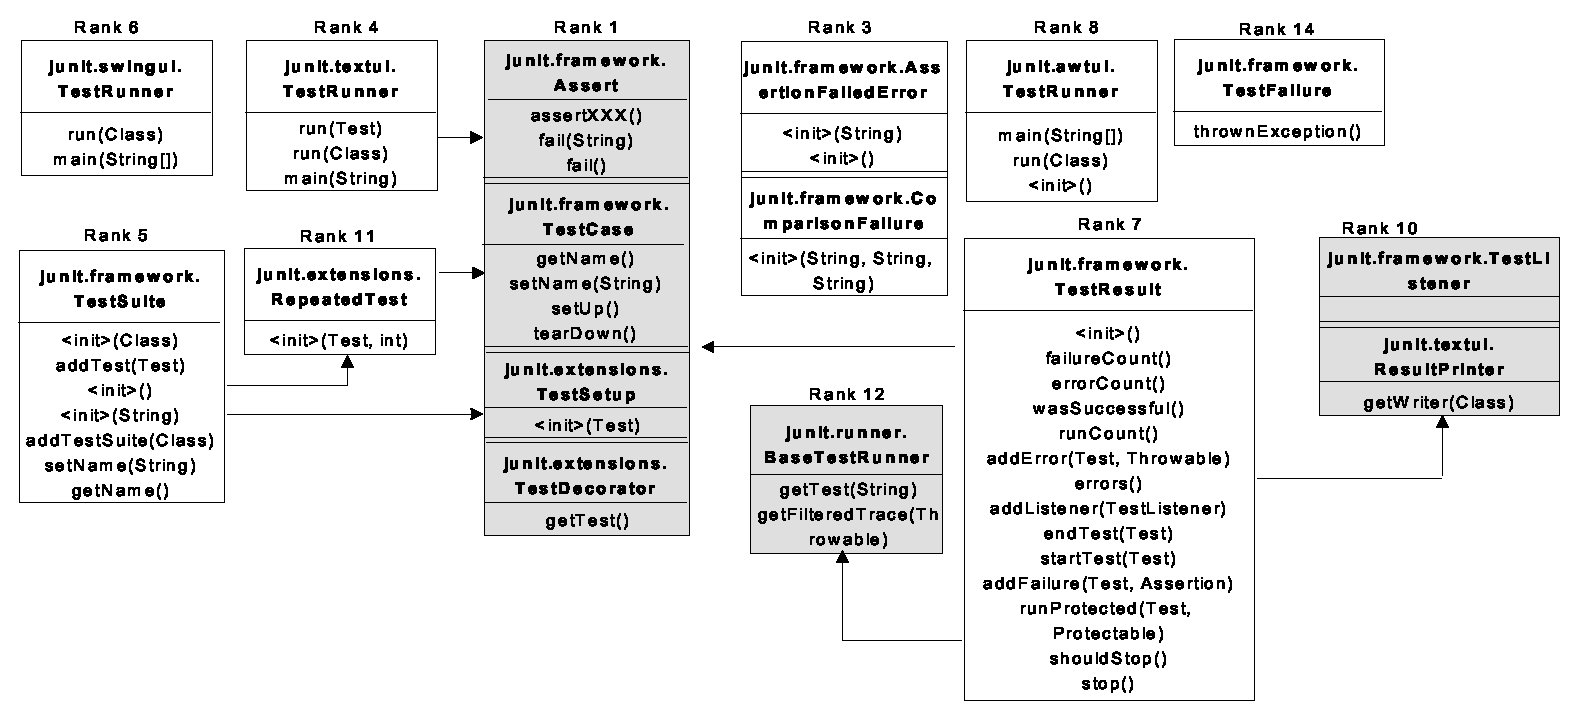
\includegraphics[scale=0.68,clip]{figs/examplehotspot_final.eps}
\caption{Hotspot hierarchies identified for the JUnit framework} \label{fig:hotspotexample}
\end{figure*}

We next use an example to explain our approach and show how the detected
hotspots and coldspots can be used by the framework users. We use JUnit~\cite{JUNIT}, the
\emph{de facto} standard unit testing framework for Java, 
as an illustrative example for explaining our approach.

SpotWeb accepts an input framework, say JUnit, and extracts
\emph{FrameworkInfo} from the framework. The
\emph{FrameworkInfo} includes all classes, all interfaces, public
or protected methods of each class and interface, and inheritance
hierarchy among classes or interfaces of the framework. SpotWeb also captures
the constants defined by the input framework. SpotWeb
constructs different queries for each class or interface and
interacts with a CSE such as Google code search~\cite{GCSE} to
gather relevant code examples from existing open source projects that
reuse the classes of the input framework. For example, SpotWeb constructs
a query such as ``\CodeIn{lang:java junit.framework.TestSuite}'' for
gathering relevant code examples of the \CodeIn{TestSuite} class. These
gathered code examples are referred as a \emph{LocalRepository} for
the input framework. SpotWeb analyzes gathered code examples
statically and computes \emph{UsageMetrics} for classes, interfaces,
and public or protected methods of all classes and interfaces. For
example, the \emph{UsageMetrics} computed for the \CodeIn{TestSuite}
class show that the class is instantiated for 165 times and is
extended for 32 times. Similarly, the \emph{UsageMetrics} computed
for the method \CodeIn{addTest} of the \CodeIn{TestSuite} class show
that the method is invoked for 95 times. SpotWeb also gathers code
examples for each class or method and stores these code examples in
a repository, referred as \emph{ExampleDB}. Then SpotWeb uses the
algorithm shown in Figure~\ref{alg:hotspotalgo} for detecting
hotspots from the computed \emph{UsageMetrics}.

Initially, SpotWeb ranks methods in a non-ascending order based on
their \emph{UsageMetrics} and uses a threshold percentage $HT$ to
detect hotspot methods: the methods in the top $HT$ percentage with
a non-zero \emph{UsageMetrics} are detected as hotspot methods. 
The detected hotspot methods are then
grouped into their declaring classes, detected as hotspot classes.
These hotspot classes are ranked based on the minimum rank of the
hotspot methods declared by these classes. SpotWeb classifies the
hotspot classes into two categories (templates and hooks) based on
heuristics described in Step 4 of the algorithm shown in Figure~\ref{alg:hotspotalgo}. The hotspot classes of each
category are further grouped into hierarchies based on their
inheritance relationships. For example, SpotWeb detected classes
\CodeIn{Assert} and \CodeIn{TestCase} as hook hotspots in the JUnit
framework. As \CodeIn{TestCase} class extends \CodeIn{Assert} class,
SpotWeb groups both the classes into the same hierarchy. SpotWeb
assigns a rank to each hierarchy based on the minimum rank of the
hotspot classes contained in the hierarchy. For example, consider
that the \CodeIn{Assert} class has Rank 1 and the \CodeIn{TestCase}
class has Rank 2, then the grouped hierarchy of the
\CodeIn{Assert} and \CodeIn{TestCase} classes is assigned with Rank
1. The rank attribute uniquely identifies a hierarchy among all
other hierarchies. Hierarchies with smaller ranks have higher preference
or importance to the hierarchies with larger ranks.

Figure~\ref{fig:hotspotexample} shows the hotspot hierarchies detected for the JUnit
framework. The figure also shows ranks assigned to each hierarchy.
As the rank attribute uniquely identifies a hierarchy, we use the
rank as an identity for describing a hierarchy.
Each hierarchy includes one or more hotspot classes and is shown as pairs of class and its methods.
For example, Hierarchy 1 (hierarchy with Rank 1) has classes \CodeIn{Assert}, \CodeIn{TestCase}, \CodeIn{TestSetup},
and \CodeIn{TestDecorator}. We show template hierarchies in white and hook hierarchies in gray.
For example, Hierarchy 1 is a hook hierarchy and Hierarchy 3 is a template hierarchy.

Methods inside each class of a hierarchy are sorted
based on their computed \emph{UsageMetrics}. Sorting methods of a class
can assist the framework users in quickly identifying the methods that are often
used inside a given hotspot class. For example, consider the \CodeIn{TestSuite} class
shown in Hierarchy 5. The \CodeIn{TestSuite} class has three constructors \CodeIn{<init>(Class)},
\CodeIn{<init>()}, and \CodeIn{<init>(String)}. However, the \CodeIn{<init>(Class)} constructor
is often used compared to the other two constructors. Due to space limit,
we show all assertion methods such as \CodeIn{assertEquals} and \CodeIn{assertTrue}
of the class \CodeIn{Assert} of Hierarchy 1 as \CodeIn{assertXXX}.

The figure also displays dependencies among hotspot hierarchies
(shown as arrows between hierarchies). SpotWeb captures the
usage relationships among hotspot classes through dependencies.
For example, Hierarchy $5$ has a
\CodeIn{TEMPLATE\_HOOK} dependency with Hierarchy $1$. This
dependency indicates that to reuse methods such as \CodeIn{addTest}
of the class \CodeIn{TestSuite} in Hierarchy 5, the user has to
define a new behavior for the classes in Hierarchy $1$.

\begin{figure}[t]
\begin{CodeOut}
\begin{alltt}
01:public class SRDAOTestCase 
02:\hspace*{0.4in}extends TestCase \{
03:\hspace*{0.1in}private SRDAO dao = null;...
04:\hspace*{0.1in}public SRDAOTestCase() \{
05:\hspace*{0.3in}super(); ... 
06:\hspace*{0.1in}\}
07:\hspace*{0.1in}protected void setUp() throws Exception \{
08:\hspace*{0.3in}...
09:\hspace*{0.3in}dao = (SRDAO)context.getBean("SRDAO");
10:\hspace*{0.3in}...
11:\hspace*{0.1in}\}
12:\hspace*{0.1in}public void tearDown() throws Exception \{
13:\hspace*{0.3in}dao = null; 
14:\hspace*{0.1in}\}
15:\hspace*{0.1in}public void testF() \{ ... \}
16:\hspace*{0.1in}public void testB() \{ ... \}
17:\hspace*{0.1in}...
18:\}
\end{alltt}
\end{CodeOut}
\Caption{\label{fig:hcodeexample} Suggested code example for the hook class \CodeIn{TestCase}.}
\begin{CodeOut}
\begin{alltt}
01:public class MyTestSuite \{ 
02:\hspace*{0.1in}...
03:\hspace*{0.1in}public static Test suite() \{
04:\hspace*{0.3in}TestSuite suite = new TestSuite("axis");
05:\hspace*{0.3in}suite.addTest(new SRDAOTestCase());
06:\hspace*{0.3in}return suite;
07:\hspace*{0.1in}\}
08:\hspace*{0.1in}...
09:\}
\end{alltt}
\end{CodeOut}
\Caption{\label{fig:tcodeexample} Suggested code example for the template class \CodeIn{TestSuite}.}
\end{figure}

We next describe how the hotspots detected by SpotWeb can be used by
the framework users to reuse classes of the JUnit framework. After reviewing
the hotspots shown in Figure~\ref{fig:hotspotexample}, consider that
a framework user wants to start with the method \CodeIn{addTest} of
the template class \CodeIn{TestSuite} in Hierarchy 5.
Figure~\ref{fig:hotspotexample} shows that Hierarchy 5 of the
\CodeIn{TestSuite} class has a \CodeIn{TEMPLATE\_HOOK} dependency
with the Hierarchy 1. This dependency indicates that the user may
need to define a new behavior for the associated hook hierarchy.
SpotWeb recommends the code example shown in
Figure~\ref{fig:hcodeexample} for the hook class \CodeIn{TestCase},
which is part of Hierarchy 1. The code example exhibits several
aspects that need to be handled by the user while extending the
\CodeIn{TestCase} class. For example, in the \CodeIn{setUp} method,
the user can write code for setting up the environment such as
instantiating necessary variables, and in the \CodeIn{tearDown}
method, the user can destroy the created variables. In addition, the code
example shows that names of the test methods in the extended class
of the \CodeIn{TestCase} class should start with the prefix \CodeIn{test}.
SpotWeb also recommends a code example for the \CodeIn{addTest} method and
the recommended code example is shown in
Figure~\ref{fig:tcodeexample}. The code example shows that the user
has to create an instance of the \CodeIn{TestSuite} class and then
add test cases through the \CodeIn{addTest} method.

An API class or method is identified as a coldspot if that class or method is neither
used directly nor used indirectly by gathered code examples. The complete
algorithm used for detecting coldspots is shown in Figure~\ref{alg:coldspotalg}. SpotWeb identified $20$
classes such as \CodeIn{Swapper}, \CodeIn{TestRunListener}, and \CodeIn{ExceptionTestCase} as coldspots
in the JUnit framework. However, coldspots are only suggestions
for users unfamiliar to that framework and SpotWeb does not intend to recommend users not to reuse
those coldspot classes. Sometimes, coldspots can also be helpful to
the framework developers in distributing their maintenance efforts, because the framework
developers can give a low preference to the coldspot classes.

\section{Approach}
\label{sec:approach}
\begin{figure}[t]
\centering
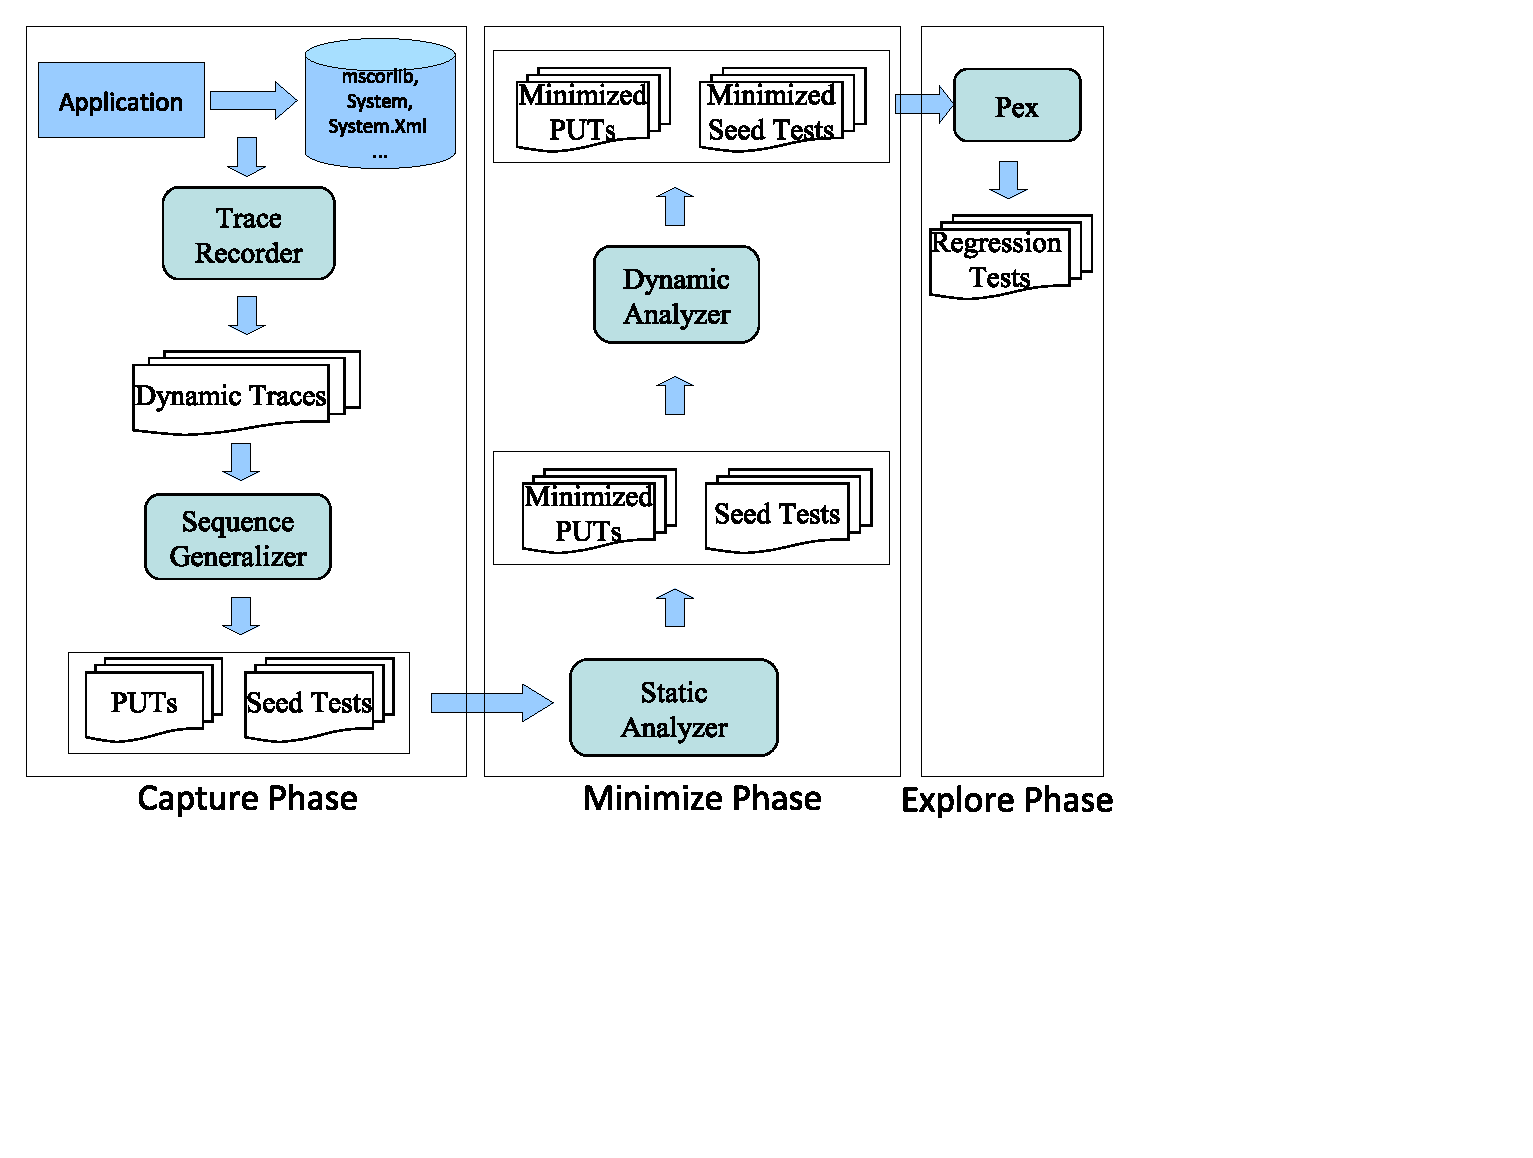
\includegraphics[scale=1,clip]{figure/approach.eps}\vspace*{-3ex}
 \caption{Overview of TeMaAPI}\vspace*{-4ex}
 \label{fig:approach}
\end{figure}
Given a migration tool between Java and C\#, TeMaAPI generates various test cases to reveal different behaviors of the tool's API mapping relations.
Figure~\ref{fig:approach} shows the overview of TeMaAPI.


%-------------------------------------------------------------------
\subsection{Generating client code}
\label{sec:approach:generating}
Given a migration tool, TeMaAPI first extracts its validate mapping relations of APIs. It is challenging to extract such mapping relations directly from a migration tool for two factors: (1) different migration tools may follow different styles to describe API mapping relations. For example, as shown in Section~\ref{sec:introduction}, the API mapping relations of Java2CSharp are described in its mapping files, but the API mapping relations of sharpen are hard-coded in its source files. (2) commercial migration tools typically hide their API mapping relations in binary files. Due to the two factors, TeMaAPI does not extract API mapping relations directly from a migration tool, but chooses to analyze translated code of a migration tool. We choose to use migration tools to translate simple client code instead of existing projects for two considerations: (1) Existing projects typically use quite a small set of APIs, so many API mapping relations may be not covered; (2) a single method of an existing project may use multiple APIs, so it may be difficult to analyze which APIs are not mapped. For the preceding consideration, TeMaAPI chooses to generate client code instead of using existing client code.

TeMaAPI relies on the reflection technique~\cite{maes1987concepts} provided by both Java and C\# to generate client code for translation.

\textbf{Static fields.} Given a public static field \CodeIn{f} of a class \CodeIn{C} whose type is \CodeIn{T}, TeMaAPI generates a getter as follows:
\begin{CodeOut}%\vspace*{-2ex}
\begin{alltt}
 public T TestGet|f.name||no|()\{ return C.f; \}
\end{alltt}
\end{CodeOut}

If \CodeIn{f} is not a constant, TeMaAPI generates a setter as follows:
\begin{CodeOut}%\vspace*{-2ex}
\begin{alltt}
 public void TestSet|f.name||no|(T v)\{ C.f = v; \}
\end{alltt}
\end{CodeOut}

\textbf{Non-static fields.} Given a public non-static field \CodeIn{f} of a class \CodeIn{C} whose type is \CodeIn{T}, TeMaAPI generates a getter for each constructor \CodeIn{C(T1\ p1,\ldots, Tn\ pn)} of \CodeIn{C} as follows:
\begin{CodeOut}%\vspace*{-2ex}
\begin{alltt}
 public T TestGet|f.name||no|(T1\ c1,\ldots, Tn\ cn)\{
    C obj = new C(c1,\ldots, cn);
    return obj.f; \}
\end{alltt}
\end{CodeOut}

If \CodeIn{f} is not a constant, TeMaAPI generates a setter as follows:
\begin{CodeOut}%\vspace*{-2ex}
\begin{alltt}
 public void TestSet|f.name||no|(T1\ c1,\ldots, Tn\ cn)\{
   C obj = new C(c1,\ldots, cn);
   obj.f = v; \}
\end{alltt}
\end{CodeOut}

In the preceding code, ``\CodeIn{|f.name|}'' denotes the name of \CodeIn{f}, and ``\CodeIn{|no|}'' denotes the corresponding number of generated client-code method.

\textbf{Static methods.} Given a public static method \CodeIn{m(T1\ p1,\ldots,Tn\ pn)} of a class \CodeIn{C} whose return type is \CodeIn{Tm}, TeMaAPI generates a client-code method as follows:
\begin{CodeOut}%\vspace*{-2ex}
\begin{alltt}
 public Tm Test|m.name||no|(T1\ m1,\ldots, Tn\ mn)\{
   return C.m(m1,\ldots, mn); \}
\end{alltt}
\end{CodeOut}

\textbf{Non-static methods.} Given a public non-static method \CodeIn{m(T1\ p1,\ldots,Tn\ pn)} of a class \CodeIn{C} whose return type is \CodeIn{Tm}, TeMaAPI generates a client-code method for each constructor \CodeIn{C(Tv\ pv,\ldots, Tt\ pt)} of \CodeIn{C} as follows:
\begin{CodeOut}%\vspace*{-2ex}
\begin{alltt}
 public Tm Test|m.name||no|(T1\ m1,\ldots, Tn\ mn,
                            Tv cv, \ldots, Tt ct)\{
   C obj = new C(cv,\ldots, ct);
   return obj.m(m1,\ldots, mn); \}
\end{alltt}
\end{CodeOut}

In the preceding code, ``\CodeIn{|m.name|}'' denotes the name of \CodeIn{m(T1\ p1,\ldots,Tn\ pn)}.

TeMaAPI ignores generic methods for simplicity, and organizes all generated client code methods by the corresponding class $C$. For a migration tool that translates from Java to C\#, TeMaAPI generates client code in Java as shown by the solid line of Figure~\ref{fig:approach}, and for a migration tool that translates from C\# to Java, TeMaAPI generates client code in C\# as shown by the dotted line of Figure~\ref{fig:approach}. When TeMaAPI generates client code in C\#, it ignores \CodeIn{unsafe} and \CodeIn{delegate} methods and methods whose parameters are marked as \CodeIn{our} or \CodeIn{ref}. Java does not have corresponding keywords, so there are typically no mapped methods in Java for these C\# methods. After TeMaAPI generate client-code methods, we translate them using a migration tool under experiments.


%-----------------------------------------------------------------
\subsection{Analyzing Generated Methods}
\label{sec:approach:analyzing}
Translated code typically contain many compilation errors since a migration tool typically cannot cover mapping relations of all APIs. TeMaAPI then analyzes translated code for validate API mapping relations of the migration tool. To achieve this, TeMaAPI first remove all translated methods with compilation errors. For translated methods in Java, TeMaAPI implements a Eclipse plug-in that uses on Eclipse JDT compiler\footnote{\url{http://www.eclipse.org/jdt/}} for the list of compilation errors. For translated methods in C\#, TeMaAPI implements a Visual Studio.Net add-in to retrieve the list of compilation errors from the error-list view of Visual Studio.Net. Both Eclipse JDT compiler and Visual Studio.Net cannot list all methods with compilation errors in a single build. After each iteration of removing methods, TeMaAPI re-build these methods until it removes all methods with compilation errors.

After methods with compilation errors are removed, TeMaAPI compares generated code with translated code for the validate API mapping relations of a migration tool. Based on translated code and validate API mapping, TeMaAPI removes generated methods whose corresponding translated methods have compilation errors. We refer to those removing client-code methods as safe methods.

%-----------------------------------------------------------
\subsection{Finding Different Behaviors}
\label{sec:approach:behavior}
In the final step, TeMaAPI generates test cases to detect different behaviors of API mapping relations. An alternative approach is to use existing test cases in two languages. For example, lucene\footnote{\url{http://lucene.apache.org}} has both a Java version and a C\# version. It is feasible to use these test cases to reveal some different behaviors, but such test cases typically cover only a small set of APIs. Some test suites such as Java Compatibility Kit (JCK)\footnote{\url{http://jck.dev.java.net}} cover most APIs of a language. However, translating such a test suite from one language into another language may introduce many compilation errors and defects. A test method may use many APIs, so even if the API under test can be translated correctly, the test method cannot be translated correctly since other APIs are not mapped. As a result, we choose to translating existing test suites as a supplement of our approach.

\subsubsection{Generating Test Cases}
\label{sec:approach:behavior:generating}
For each safe method in Java, we use Randoop~\cite{pacheco2007feedback} to generate its test cases. For each safe method in C\#, we use Pex~\cite{tillmann2008pex} to generate its test cases. TeMaAPI then executes generated test cases, and records the inputs, the output, and the thrown exception of each test case as a file.

Based on the file, TeMaAPI generates Junit\footnote{\url{http://www.junit.org/}} or Nunit\footnote{\url{http://www.nunit.org/}} test cases to ensure each mapped API produce the same output give the same inputs. For example, Pex generates a test case whose input is \CodeIn{m0 = false} for the \CodeIn{TestvalueOf57} method in C\# as shown in Section~\ref{sec:example}, and after executing the output of the test case is ``False''. Based on the input and the output of this test case, TeMaAPI generates a Junit test case as follows:

\begin{CodeOut}%\vspace*{-2ex}
\begin{alltt}
 @Test
 public void testvalueOf64zhh0()\{
   sketch.Test_java_lang_String obj =
                       new sketch.Test_java_lang_String();
   boolean m0 = false;
   Assert.assertEquals("False", obj.testvalueOf64(m0));\}
\end{alltt}
\end{CodeOut}

This Junit test case fails since the preceding \CodeIn{testvalueOf64zhh} method produces ``false'' instead of ``False''. From this failed Junit test case, TeMaAPI detects that the \CodeIn{java.lang.String.valueOf (Object)} method in Java has different behaviors with its mapped C\# methods if inputs are boolean values.

In some cases, executing a test case does not produce outputs but exceptions. For example, Pex also generates a test case whose input is \CodeIn{m0 = null} for the \CodeIn{TestvalueOf57} method in C\# as shown in Section~\ref{sec:example}, after executing it throws \CodeIn{NullReferenceException}. TeMaAPI finds that the \CodeIn{NullPointerException} class in C\# is mapped to the \CodeIn{NullPointerException} class in Java in the validate API mapping relations, and generates a Junit test case based on the preceding mapping relation and input as follows:

\begin{CodeOut}%\vspace*{-2ex}
\begin{alltt}
 @Test
 public void testvalueOf64zhh3()\{
   try\{
     sketch.Test_java_lang_String obj =
                       new sketch.Test_java_lang_String();
     boolean m0 = null;
     obj.testvalueOf64(m0);\}
   \}catch(java.lang.NullPointerException e)\{
       Assert.assertTrue(true);
       return;
   \}
   Assert.assertTrue(false);\}
\end{alltt}
\end{CodeOut}

This Junit test case also fails since given a null input, the preceding \CodeIn{testvalueOf64} method does not throw any exceptions. From this failed Junit test case, TeMaAPI detects that the \CodeIn{java.lang. String.valueOf(Object)} method in Java has different behaviors with its mapped C\# methods if inputs are null pointers.

\subsubsection{Translating Existing Test Cases}
\label{sec:approach:behavior:jck}

Each generated client-code method uses only one fields or methods provided by API libraries, and may lose some complicated behaviors even if test cases satisfy the round-trip criterion. To test those complicated behaviors, we introduce JCK that covers many complicated behaviors of Java APIs. JCK is a test suite provided by Sun to ensure compatibility of Java platforms, and it covers most standard APIs of J2SE. However, JCK implements many internal classes to collect the results of executed test cases. If a migration tool cannot correctly translate one of these classes, all translated test cases may have compilation errors or defects. In addition, JCK is released under read-only source license\footnote{\url{http://tinyurl.com/33x9fo6}}, so many such internal classes are not shipped and it has many compilation errors. To increase the chance of migrating JCK, TeMaAPI first replaces those internal classes with the classes of Junit. For example, one test method for \CodeIn{java.io.File.delete()} in JCK is as follows:

\begin{CodeOut}%\vspace*{-2ex}
\begin{alltt}
  public Status File0037()\{
    String testCaseID = "File0037";
    ...
    FileRT method = new FileRT(testCaseID) \{
     public Status run() \{
       File f = null;
       f = new File(workdir, testCaseID);
       ...
       if (f.delete()) \{ // Try to delete
         if (!f.exists()) \{ // Does it exist?
           return Status.passed("OKAY");
         \}else\{
            return Status.failed(...);
         \}
       else\{
           return Status.failed(...);
       \}
    \}
     return AllPermissionSM.testRun(...);
  \}
\end{alltt}
\end{CodeOut}

After the preceding three steps, TeMaAPI further replaces the statement starts with \CodeIn{FileRT} with the body of the \CodeIn{run} method, and removes the last statement. The translated code is as follows:

\begin{CodeOut}%\vspace*{-2ex}
\begin{alltt}
  public void File0037()\{
    String testCaseID = "File0037";
    ...
    File f = null;
    f = new File(workdir, testCaseID);
    ...
    if (f.delete()) \{ // Try to delete
      if (!f.exists()) \{ // Does it exist?
        Assert.assertTrue(true);
        return;
     \}else\{
        Assert.fail();
        return;
     \}
   else\{
       Assert.fail();
       return;
   \}
  \}
\end{alltt}
\end{CodeOut}

Compared with the original test method in JCK, the translated method does not use the three internal classes: \CodeIn{Status}, \CodeIn{FileRT}, and \CodeIn{AllPermissionSM}. 

After the preceding process, for a migration tool, TeMaAPI further removes methods that use any APIs outside its defined mapping relations. The remaining methods can be translated from Java to other languages since it does not use any APIs outside of the migration tool.



\section{Evaluation}
\label{sec:eval}

We conducted three different evaluations to show the effectiveness of our $\smoot$ approach. In our evaluations, we used two popular .NET applications: QuickGraph~\cite{QUICKGRAPH} and Facebook~\cite{FACEBOOK}. Our empirical results show that $\smoot$ handles large code bases and extracts sequences that can help achieve target states. Our empirical results also show that our approach can effectively assist random and DSE-based approaches in achieving higher branch coverage. The details of subjects and results of our evaluation are available at \url{http://research.csc.ncsu.edu/ase/projects/mseqgen/}. \\ All experiments were conducted on a machine with 1.6GHz Xeon processor and 1GB RAM. We next present research questions addressed in our evaluations.

%------------------------------------------------------------------------
\subsection{Research Questions}

In our evaluations, we address the following research questions.\vspace*{-1ex}

\begin{itemize}
\item RQ1: Can our approach handle large code bases in gathering sequences for target classes of subject applications?
\item RQ2: Can our approach assist a random approach in achieving higher code coverage of the code under test than without the assistance of our approach?
\item RQ3: Can our approach assist a DSE-based approach in achieving higher code coverage of the code under test than without the assistance of our approach?
\end{itemize}

%------------------------------------------------------------------------
\subsection{Subject Applications}

We used two popular .NET applications for evaluating our $\smoot$ approach: QuickGraph~\cite{QUICKGRAPH} and Facebook~\cite{FACEBOOK}. QuickGraph is a C\# graph library that provides various directed/undirected graph data structures. QuickGraph also provides algorithms such as depth-first search, breadth-first search, and A* search~\cite{thomas:algos}. 
QuickGraph includes 165 classes and interfaces with 5 KLOC. Facebook is a popular social network website that connects people with friends and others whom they work, study, and live around. In our evaluation, we use a Facebook developer toolkit that provides APIs necessary for developing Facebook applications. The Facebook developer toolkit includes 285 classes and interfaces with 40 KLOC.

%------------------------------------------------------------------------
\subsection{RQ1: Gathering Sequences}

We next address the first research question on whether our approach can handle large code bases in gathering sequences for target classes of the QuickGraph and Facebook applications. For QuickGraph and Facebook, we use code bases including 3.85 MB and 5 MB of .NET assembly code, respectively. Our approach extracted 167 sequences for QuickGraph with a maximum length of 12 method calls for the \CodeIn{AdjacencyGraph} class. Our approach took 5.2 minutes for analyzing code bases related to QuickGraph. For Facebook, our approach extracted 355 sequences with a maximum length of 51 method calls for the \CodeIn{Hashtable} class.  Although the sequence extracted for \CodeIn{Hashtable} is long, this sequence includes method calls such as \CodeIn{Add} for multiple times. Our approach took 4.5 minutes for analyzing code bases related to Facebook and to gather these sequences. Our results show that our approach can mine large code bases for gathering sequences to help achieve target states.

%------------------------------------------------------------------------
\subsection{RQ2: Assisting Random Approach}

We next address the second research question on whether our approach helps increase branch coverage achieved by a state-of-the-art random approach, called Randoop~\cite{pacheco:feedback}. To address this research question, we first run Randoop on QuickGraph and Facebook applications, and generate test inputs. Randoop generates test inputs in the form of sequences of method calls. We execute generated test inputs and measure branch coverage using a coverage measurement tool, called NCover\footnote{\url{http://www.ncover.com/}}. This measured coverage forms a baseline for comparing Randoop with and without the assistance from our approach. In our evaluation, we use default configurations provided by the Randoop developers. For each namespace of the subject application, we ran Randoop for a maximum of 130 seconds.

To assist Randoop with our extracted sequences, we synthesize static method bodies that include our gathered sequences and return objects of target classes of our subject applications. For example, if a target class $TC_j$ has four sequences, we synthesize four static method bodies where each method body returns an object of $TC_j$ by executing a gathered sequence for $TC_j$. If a sequence for $TC_j$ requires other objects of non-primitive or primitive types (whose values are not known in gathered sequences due to static analysis), we add those non-primitive and primitive types as arguments for the method bodies. For primitive types, Randoop randomly generates some values. For non-primitive types, Randoop randomly generates a new sequence or selects some other method body (synthesized by our approach) that produces that non-primitive type. We gather newly generated test inputs that include the method bodies synthesized by $\smoot$ and add these new test inputs to existing tests to measure the increase in the branch coverage. 

\setlength{\tabcolsep}{1pt}
\begin{table*}[t]
\begin{SmallOut}
\begin{CodeOut}
\begin{center}
\begin {tabular} {|l|c|c|c|c|c|}
\hline
\textbf{Application} & \textbf{\#} of & \textbf{Test Code} & \textbf{Random} & \textbf{Random + $\smoot$} & \textbf{\% Increase in }\\
 & \textbf{classes} & \textbf{T} & \textbf{R} & \textbf{R + M} & \textbf{Branch coverage}\\
\hline
\hline QuickGraph.Algorithms & 104 & 18.4 & 63.3 & 63.3 & - \\
\hline QuickGraph.Algorithms.Search & 11 & 40.3 & 33.3 & 47.6 & \textbf{14.3} \\
\hline QuickGraph.Algorithms.ShortestPath & 4 & 0 & 29.3 & 30.2 & 0.9 \\
\hline QuickGraph.Algorithms.Visitors & 11 & 0 & 86.4 & 86.4 & - \\
\hline QuickGraph.Collections & 19 & 11.2 & 74.0 & 83.3 & 9.3 \\
\hline QuickGraph.Exceptions & 3 & 40.0 & 100.0 & 100.0 & - \\
\hline QuickGraph.Predicates & 9 & 8.6 & 43.1 & 48.3 & 5.2 \\
\hline QuickGraph.Providers & 1 & 100.0 & 80.0 & 100.0 & \textbf{20.0} \\
\hline QuickGraph.Representations & 3 & 43.1 & 35.1 & 49.0 & \textbf{13.9} \\
\hline facebook & 25 & 48.9 & 14.0 & 23.3 & 9.3 \\
\hline facebook.Components & 3 & 0 & 30.7 & 30.7 & - \\
\hline facebook.desktop & 14 & 0 & 18.5 & 21.0 & 2.5 \\
\hline facebook.Forms & 4 & 0 & 11.1 & 11.1 & - \\
\hline facebook.Properties & 1 & 31.3 & 37.5 & 37.5 & - \\
\hline facebook.Schema & 216 & 6.1 & 20.8 & 24.8 & 4.1 \\
\hline facebook.Types & 1 & 0 & 100.0 & 100.0 & - \\
\hline facebook.Utility & 8 & 49.1 & 22.6 & 37.7 & \textbf{15.1} \\
\hline facebook.web & 12 & 0 & 3.3 & 4.5 & 1.2 \\
%\hline \textbf{AVERAGE} &  & 22 & 44.61 & 49.92 &  \\
\hline \textbf{AVERAGE} &  &  &  &  & \textbf{8.7} \\
\hline
\end{tabular}
\end{center}
\end{CodeOut}
\end{SmallOut}\vspace*{-4ex}
\centering \caption {\label{tab:premresults} Evaluation results showing higher branch coverage achieved by Randoop with the assistance of $\smoot$. \CodeIn{T: Test code, R: Randoop, M: $\smoot$}}
\end{table*}

Table~\ref{tab:premresults} shows the results of our evaluation with both subject applications. The table shows the results for all namespaces of the subject applications. As we include test code available with subject applications in code bases used for extracting sequences, we show branch coverage achieved by the test code alone in Column ``T''. Column ``R'' shows branch coverage achieved by Randoop. Column ``R + M'' shows branch coverage achieved by Randoop with the assistance of our $\smoot$ approach. Column ``Increase in Branch Coverage'' shows additional branch coverage achieved with the assistance from our $\smoot$ approach. As shown in our results, ``R + M'' achieved higher coverage than Randoop and test code (except for namespaces \CodeIn{facebook} and \CodeIn{facebook.Utility}). There are two primary reasons for lower coverage of ``R + M'' for these two namespaces: the random mechanism of Randoop and limitations of our current implementation. Due to the random mechanism used by Randoop, various method calls used in test code that contributed to higher coverage achieved by the test code are not used by Randoop in generating test inputs. Section~\ref{sec:future} presents limitations of our current implementation on why ``R + M'' achieved lower coverage than existing test code for namespaces \CodeIn{facebook} and \CodeIn{facebook.Utility}. Our results show that there is a considerable increase of 8.7\% on average\footnote{We compute average from those namespaces that have a non-zero increase in the branch coverage} (with a maximum of 20\%) in branch coverage achieved by Randoop with assistance from our approach. 

\begin{figure}[t]
\begin{CodeOut}
\begin{alltt}
00:class BidirectionalGraph \{ ...
01:\hspace*{0.1in}public IEdge AddEdge(IVertex src, IVertex tg) \{
02:\hspace*{0.2in}// look for the vertex in the list
03:\hspace*{0.2in}if (!VertexInEdges.ContainsKey(src))
04:\hspace*{0.3in}throw new VertexNotFoundException 
\hspace*{0.5in}("Could not find source");
05:\hspace*{0.2in}if (!VertexInEdges.ContainsKey(tg))
06:\hspace*{0.3in}throw new VertexNotFoundException 
\hspace*{0.5in}("Could not find target");
07:\hspace*{0.2in}// create edge
08:\hspace*{0.2in}IEdge e = base.AddEdge(src, tg);
09:\hspace*{0.2in}VertexInEdges[target].Add(e);
10:\hspace*{0.2in}return e;
11:\hspace*{0.1in}\}
12:\}
\end{alltt}
\end{CodeOut} \vspace*{-5ex}
\Caption{\label{fig:vidMUT} A MUT \CodeIn{AddEdge} in the \CodeIn{BidirectionalGraph} class of QuickGraph.} \vspace*{-5ex}
\end{figure}

We next provide examples to describe scenarios where our approach can assist random approaches. We also describe scenarios where our approach cannot assist random approaches. We use a MUT, called \CodeIn{AddEdge}, in the \CodeIn{BidirectionalGraph} class of the \CodeIn{QuickGraph.Representations} namespace (shown in Figure~\ref{fig:vidMUT}). Although Randoop generated three test inputs (in the form of sequences) for the \CodeIn{AddEdge} MUT, Randoop achieved low branch coverage of 40.0\% (2 out of 5 branches). The reason for not achieving high coverage for the \CodeIn{AddEdge} MUT is that the \CodeIn{AddEdge} MUT requires a specific receiver object state. To reach Statement 8 of the MUT, the \CodeIn{VertexInEdges} field should include the new vertices represented by \CodeIn{src} and \CodeIn{tg} that are passed as arguments. With the sequences extracted by our approach, Randoop achieved a branch coverage of 80.0\% (4 out of 5 branches). As our sequences are extracted from code bases that include usage scenarios on how these method calls are used in real practice, our sequences helped achieve high coverage for the \CodeIn{AddEdge} MUT. 

Although Randoop achieved higher branch coverage with the assistance from our approach, the test inputs generated by Randoop did not cover the \CodeIn{true} branch of Statement 5 to reach Statement 6. The reason is that our sequences do not include a usage scenario where the \CodeIn{AddEdge} MUT is invoked with one vertex in \CodeIn{VertexInEdges} and the other vertex not in \CodeIn{VertexInEdges}. Such usage scenarios rarely exist in code bases that are used for extracting sequences as these usage scenarios are related to testing the MUT for negative cases rather than reusing the MUT in real practice. However, a more systematic approach such as a DSE-based approach can cover such not-covered branches with the assistance from our approach.

%------------------------------------------------------------------------
\subsection{RQ3: Assisting DSE-based Approaches}

We next address the third research question on whether our approach can help increase branch coverage achieved by a DSE-based approach. To address this research question, we use a state-of-the-art DSE-based approach called Pex~\cite{tillman:pexwhite}. Pex accepts PUTs as input and generates conventional unit tests from these PUTs using DSE. As PUTs are not available with our subject applications, we generated PUTs for each public method in our subject applications using the \emph{PexWizard} tool. PexWizard is a tool provided with Pex and this tool automatically generates PUTs for each public method in the application given as input. A PUT generated for the \CodeIn{Compute} MUT (Figure~\ref{fig:mut}) is shown below.

\begin{CodeOut}
\begin{alltt}
00:[PexMethod]
01:public void Compute01(
02:\hspace*{0.3in}[PexAssumeUnderTest]UndirectedDFS target,
03:\hspace*{0.3in}[PexAssumeUnderTest]Vertex s) \{
04:\hspace*{0.1in}target.Compute(s);
05:\hspace*{0.1in}Assert.Inconclusive("this test has to be reviewed");
06:\}
\end{alltt}
\end{CodeOut}

The receiver object and argument objects required for the \CodeIn{Compute} MUT are accepted as arguments for the PUT. Pex generates skeletons for the non-primitive arguments by using a heuristic-based approach (Section~\ref{sec:pex}). For this evaluation, we used only the QuickGraph application. The reason is that Pex does not terminate in generating unit tests for the Facebook application. In future work, we plan to investigate the issues with Pex and apply Pex on the Facebook application. To provide a baseline for showing the effectiveness of our approach, we first applied Pex on PUTs generated for the QuickGraph application. We executed generated unit tests and measured branch coverage achieved by these unit tests for different namespaces in the QuickGraph application. In our evaluation, we use default configurations of Pex.

We next used our extracted sequences to assist Pex. Pex provides a feature called \emph{factory} methods, which allow programmers to provide assistance to Pex in generating non-primitive object types. We used this feature by converting our extracted sequences into factory methods. One issue with factory methods is that the current Pex allows only one factory method for a non-primitive object type. As our approach can extract multiple sequences for creating an object of a non-primitive type, we combine all sequences related to a non-primitive type into one factory method by using a \CodeIn{switch} statement. We next apply Pex on the subject application with new factory methods created based on our extracted sequences. We again generate unit tests using Pex and measure new branch coverage. 

\setlength{\tabcolsep}{1pt}
\begin{table}[t]
\begin{SmallOut}
\begin{CodeOut}
\begin{center}
\begin {tabular} {|l|c|c|c|c|}
\hline
\textbf{Application} & \textbf{\# C} & \textbf{P} & \textbf{P + M} & \textbf{Increase}\\
 &  &  &  & \textbf{\%}\\
\hline
\hline QuickGraph.Algorithms & 104 & 8.2 & 30.6 & \textbf{22.5}\\
\hline QuickGraph.Algorithms.Search & 11 & 0 & 13.9 & \textbf{13.9}\\
\hline QuickGraph.Algorithms.ShortestPath & 4 & 1.9 & 1.9 & -\\
\hline QuickGraph.Algorithms.Visitors & 11 & 50.0 & 50.0 & -\\
\hline QuickGraph.Collections & 19 & 14.9 & 29.0 & \textbf{14.1}\\
\hline QuickGraph.Exceptions & 3 & 60.0 & 60.0 & -\\
\hline QuickGraph.Predicates & 9 & 31.0 & 31.0 & -\\
\hline QuickGraph.Representations & 1 & 2.7 & 21.6 & \textbf{19.2}\\
\hline \textbf{AVERAGE} &  & & & \textbf{17.4}\\
\hline
\end{tabular}
\end{center}
\end{CodeOut}
\end{SmallOut}\vspace*{-4ex}
\centering \caption {\label{tab:pexresults} Evaluation results showing higher branch coverage achieved by Pex with the assistance of $\smoot$. \CodeIn{\# C: number of classes, P: Pex, M: $\smoot$}}\vspace*{-3ex}
\end{table}

Table~\ref{tab:pexresults} shows our results by applying Pex with and without our sequences on the QuickGraph application. On average, our approach helped increase the branch coverage by 17.4\% (with a maximum increase of 22.5\% for one namespace). Although there is a considerable increase in branch coverage with the assistance from our approach, overall Pex still achieved low branch coverage. This result is due to a limitation with the current Pex that cannot automatically identify implementing classes for interfaces and use their related factory methods. Often, factory methods created by our approach accept interfaces as arguments. Therefore, Pex is not able to identify relevant factory methods for interfaces, although factory methods for their implementing classes are created by our approach. In future work, we plan to address this limitation and we expect that our results can be much better after addressing this limitation of Pex.

We next present example scenarios where our approach is quite useful in achieving higher branch coverage with Pex. We use the  \CodeIn{TopologicalSortAlgorithm} class in the \CodeIn{QuickGraph.Algorithms} namespace as an illustrative example. Without the assistance from our approach, Pex did not achieve any coverage of the \CodeIn{TopologicalSortAlgorithm} class as Pex was not able to generate any sequences for creating objects of the \CodeIn{TopologicalSortAlgorithm} class. The reason for not able to generate any sequences is that the constructor of \CodeIn{TopologicalSortAlgorithm} accepts an interface as input. Using the factory methods generated by our approach, Pex achieved a branch coverage of 57.9\% (11 out of 19 branches). Our results show that our approach can assist DSE-based approaches in achieving higher code coverage than without using our approach.

%TODO: *. You should emphasize the improving the branch coverage achieved by Randoop or Pex is not trivial. The remaining not-covered branches are challenging to cover. See some arguments from the Evacon paper. Some reviewers may say that improvement of 15% or 20% is not a big deal. We want to argue against them before they speak out.


\section{Threats to Validity}
\label{sec:threats}
The threats to external validity primarily include the degree to which the subject programs and used CSE are representative of true practice. The current subjects range from small-scale libraries such as Java SQL APIs to large-scale libraries such as BCEL and Hibernate. We used only one CSE, i.e., Google code search, which is a well-known CSE. These threats could be reduced by more experiments on wider types of subjects and by using other CSEs in future work. The threats to internal validity are instrumentation effects that can bias our results. Faults in our Alattin prototype might cause such effects. There can be errors in our inspection of source code for confirming rules or defects. To reduce these threats, we inspected available specifications and also call sites in source code.
\section{Discussion and Future Work}
\label{sec:future}

Although random and DSE-based approaches show considerable increase in branch coverage with the assistance from our approach, overall coverage achieved by these approaches are still not close to 100\% coverage. The reason is that often code under test includes complex branches that are quite difficult to cover. We next give an example of a difficult branch that is not covered by any of the approaches used in our evaluation. We use the code example shown in Figure~\ref{fig:diffbranch} as an illustrative example. This difficult branch is in the \CodeIn{Visit} method of the \CodeIn{BreadthFirstSearchAlgorithm} class. The receiver-object state to reach Statement 8 requires that the \CodeIn{VisitedGraph} object has a non-empty set of vertices and edges. Reaching Statement 8 also requires a specific object state for the argument \CodeIn{s}. In particular, the vertex represented by the argument \CodeIn{s} should already exist in the \CodeIn{VisitedGraph} object and should have outgoing edges. Although our extracted sequences include a sequence for achieving a desirable receiver-object state, our sequences do not include a necessary sequence for achieving a desirable argument-object state. In future work, we plan to further address these issues by generating new sequences using evolutionary approaches~\cite{tonella:etoc,  inkumsah08:improving}. There, we can use our extracted sequences as an initial set for these evolutionary approaches to evolve. Generation of new sequences using evolutionary approaches can also help reduce the bias in our approach, where our approach gives more preference to verify common usage rather than uncommon usage.

\begin{figure}[t]
\begin{CodeOut}
\begin{alltt}
00:public void Visit(IVertex s) \{
01:\hspace*{0.1in}...
02:\hspace*{0.1in}m\_Q.Push(s);
03:\hspace*{0.1in}while (m\_Q.Count != 0) \{
04:\hspace*{0.2in}IVertex u = (IVertex)m\_Q.Peek(); 
05:\hspace*{0.2in}m\_Q.Pop();
06:\hspace*{0.2in}...
07:\hspace*{0.2in}foreach(IEdge e in VisitedGraph.OutEdges(u)) \{ 
08:\hspace*{0.3in}...		//Difficult branch
09:\hspace*{0.2in}\} 
10:\hspace*{0.1in}\}
11:\}
\end{alltt}
\end{CodeOut}\vspace*{-5ex}
\Caption{\label{fig:diffbranch} An example difficult branch not reached by any approach used in our evaluation.}\vspace*{-5ex}
\end{figure}

In our evaluations, for the \CodeIn{facebook} and \CodeIn{facebook.Utility} namespaces, branch coverage achieved by Randoop (with the assistance of our approach) is lower than branch coverage achieved by the test code (commonly written by  application developers). There are two primary reasons for lower coverage of these namespaces: limitations of the random mechanism of Randoop and our current implementation. Our current implementation does not handle several features such as inheritance or C\# generics. Therefore, our implementation could not capture some sequences due to their use of these features. In future work, we plan to extend our implementation to support these features. 

%In our current approach, gathering sequences is loosely coupled with dynamic symbolic execution. For example, we identify the target classes and gather method-call sequences from code bases. We next verify whether these sequences can help achieve the $\theta$ states. Therefore, some collected sequences can be irrelevant. In future work, we plan to identify a desirable target (such as a branch) that is not achieved by the dynamic symbolic execution and use that information to gather sequences. This additional information can help gather more relevant sequences. 

Our approach extracts sequences from code bases using the receiver or argument object types of a MUT (in a framework under analysis) and generates method bodies to assist test-generation approaches. Sometimes, these sequences may include object types specific to the code bases. For example, these object types can be classes that implement interfaces provided by the framework under analysis. In such scenarios, the method bodies generated by our approach are not compilable. Currently, we fix those compilation errors manually. In future work, we plan to automatically compile and verify extracted sequences to reduce this manual effort.

\Comment{We currently gather \emph{only} one path from a CFG to generate sequences. However, there can be different sequences
across multiple paths in the CFG. In future work, we plan to collect sequences from multiple paths in the CFG. We also plan to develop clustering heuristics to cluster similar sequences.}


\section{Related Work}
\label{sec:related}

Our approach is related to previous work on two areas:
language translation and library migration.

\textbf{Language translation.} To reduce manual efforts of language
translation~\cite{samet1981experience}, researchers proposed various
approaches~\cite{hassan2005lightweight,van1999identifying,waters1988program,mossienko2003automated,yasumatsu1995spice} to automate the process.
However, all these approaches focus on the syntax or structural differences between
languages. Deursen \emph{et al.}~\cite{van1999identifying} proposed an approach to identify
objects in legacy code. Their approach uses these objects to deal with the
differences between object-oriented and procedural languages. As
shown in El-Ramly \emph{et al.}~\cite{el2006experiment}'s experience
report, existing approaches support only a subset of APIs for language translation,
making the task of language translation a challenging problem.
In contrast to previous approaches, our approach automatically mines API mapping between
languages to aid language translation, addressing a significant
problem not addressed by the previous approaches and complementing
these approaches.

\textbf{Library migration.} With evolution of libraries, some APIs
may become incompatible across library versions. To address this
problem, Henkel and Diwan~\cite{henkel2005catchup} proposed an approach that captures
and replays API refactoring actions to update the client code.
Xing and Stroulia~\cite{xing2007api} proposed an approach that
recognizes the changes of APIs by comparing the differences between two
versions of libraries. Balaban \emph{et al.}~\cite{balaban2005refactoring} proposed
an approach to translate client code when mapping relations of libraries are
available. In contrast to these approaches, our approach focuses on
mapping relations of APIs across different languages. In addition, since
our approach uses ATGs to mine API mapping relations, our approach can also
mine mapping relations between API methods with different parameters or between
API methods whose functionalities are split among several API methods in the other language.

\textbf{Mining specifications.} Some of our previous approaches~\cite{zhong09:inferring,zhong09:mapo,thummalapenta09:mining,thummalapenta09:mseqgen,acharya09:mining} focus on mining specifications. MAM mines API mapping relations across different languages for language migration, whereas the previous approaches mine API properties of a single language to detect defects or to assist programming.

\section{Conclusion}
\label{sec:conclusion}

API Mapping relations serve as a basis for automatic translation tools to translate applications from one language to another. However, original and translated applications can exhibit different behaviors due to inconsistencies among mapping relations. In this paper, we proposed an approach, called TeMaAPI, that detects different behaviors of mapped API methods via testing. TeMaAPI targets at generating test cases that covers all feasible paths and  sequences to reveal different behaviors of both single methods and method sequences. We implemented a tool and conducted three evaluations on five translation tools to show the effectiveness of our approach. The results show that our approach detects various differences between mapped API methods. We further analyze these differences and their implications. We expect that our results can help improve existing translation tools and help programmers better understand differences of Java and C\#.

%Mapping relations of APIs are quite useful for the migration tools, but these mapping relations also can introduce defects to translated code since mapped API methods may have different behaviors. In this paper, we propose an approach, called TeMaAPI, that detects different behaviors of mapped API methods via testing. TeMaAPI targets at generating test cases that covers all feasible paths and  sequences to reveal different behaviors of both single invocations and invocation sequences. We implemented a tool and conducted three evaluations on five migration tools to show the effectiveness of our approach. The results show that our approach detects various differences between mapped API invocations. We further analyze these differences and their implications. The results can help improve existing migration tools and help programmers better understand differences of Java and C\#.


\section*{Acknowledgments}

We thank Shuvendu Lahiri and Thomas Ball for sharing Randoop used in our evaluations.

\bibliographystyle{abbrv}
\begin{thebibliography}{10}

\bibitem{acharya06:mining}
M.~Acharya, T.~Xie, and J.~Xu.
\newblock {Mining Interface Specifications for Generating Checkable Robustness
  Properties}.
\newblock In {\em Proc. ISSRE}, pages 311--320, 2006.

\bibitem{agarwal:association}
R.~Agrawal and R.~Srikant.
\newblock Fast algorithms for mining association rules in large databases.
\newblock In {\em Proc. VLDB}, pages 487--499, 1994.

\bibitem{Clarke:symbolic}
L.~Clarke.
\newblock {A System to Generate Test Data and Symbolically Execute Programs}.
\newblock {\em IEEE Trans. Softw. Eng.}, 2(3):215--222, 1976.

\bibitem{thomas:algos}
T.~H. Cormen, C.~Stein, R.~L. Rivest, and C.~E. Leiserson.
\newblock {\em Introduction to Algorithms}.
\newblock McGraw-Hill Higher Education, 2001.

\bibitem{csallner:jcrasher}
C.~Csallner and Y.~Smaragdakis.
\newblock {JC}rasher: an automatic robustness tester for {J}ava.
\newblock {\em Softw. Pract. Exper.}, 34(11):1025--1050, 2004.

\bibitem{random:duran}
J.~Duran and M.~Ntafos.
\newblock An evaluation of random testing.
\newblock {\em IEEE Trans. Softw. Eng.}, 10(4):438--444, 1984.

\bibitem{Elbaum:capture}
S.~Elbaum, H.~N. Chin, M.~B. Dwyer, and J.~Dokulil.
\newblock {Carving differential unit test cases from system test cases}.
\newblock In {\em Proc. FSE}, pages 253--264, 2006.

\bibitem{Engler2001deviant}
D.~Engler, D.~Y. Chen, S.~Hallem, A.~Chou, and B.~Chelf.
\newblock {Bugs as deviant behavior: a general approach to inferring errors in
  systems code}.
\newblock In {\em Proc. SOSP}, pages 57--72, 2001.

\bibitem{FACEBOOK}
Facebook developer toolkit, 2008.
\newblock \url{http://www.codeplex.com/FacebookToolkit}.

\bibitem{godefroid:dart}
P.~Godefroid, N.~Klarlund, and K.~Sen.
\newblock {DART}: {D}irected automated random testing.
\newblock In {\em Proc. PLDI}, pages 213--223, 2005.

\bibitem{inkumsah08:improving}
K.~Inkumsah and T.~Xie.
\newblock Improving structural testing of object-oriented programs via
  integrating evolutionary testing and symbolic execution.
\newblock In {\em Proc. ASE}, pages 297--306, 2008.

\vfill\eject

\bibitem{JTEST}
Parasoft. {J}test manuals version 5.1. {O}nline manual, 2006.
\newblock \url{http://www.parasoft.com}.

\bibitem{khurshid:symbolic}
S.~Khurshid, C.~S. Pasareanu, and W.~Visser.
\newblock {Generalized symbolic execution for model checking and testing}.
\newblock In {\em Proc. TACAS}, pages 553--568, 2003.

\bibitem{king:symex}
J.~C. King.
\newblock {Symbolic Execution and Program Testing}.
\newblock {\em Communications of the ACM}, 19(7):385--394, 1976.

\bibitem{koushik:cute}
S.~Koushik, M.~Darko, and A.~Gul.
\newblock {CUTE: a concolic unit testing engine for C}.
\newblock In {\em Proc. ESEC/FSE}, pages 263--272, 2005.

\bibitem{Xiyang:fitness}
X.~Liu, H.~Liu, B.~Wang, P.~Chen, and X.~Cai.
\newblock {A unified fitness function calculation rule for flag conditions to
  improve evolutionary testing}.
\newblock In {\em Proc. ASE}, pages 337--341, 2005.

\bibitem{orso:capture}
A.~Orso and B.~Kennedy.
\newblock {Selective capture and replay of program executions}.
\newblock {\em SIGSOFT Softw. Eng. Notes}, 30(4):1--7, 2005.

\bibitem{pacheco:eclat}
C.~Pacheco and M.~D. Ernst.
\newblock Eclat: Automatic generation and classification of test inputs.
\newblock In {\em Proc. ECOOP}, pages 504--527, 2005.

\bibitem{pacheco:feedback}
C.~Pacheco, S.~K. Lahiri, M.~D. Ernst, and T.~Ball.
\newblock Feedback-directed random test generation.
\newblock In {\em Proc. ICSE}, pages 75--84, 2007.

\bibitem{QUICKGRAPH}
{QuickGraph: A 100\% C\# graph library with Graphviz Support, Version 2.0},
  2008.
\newblock \url{http://www.codeproject.com/KB/miscctrl/quickgraph.aspx}.

\bibitem{david:java}
D.~Saff, S.~Artzi, J.~H. Perkins, and M.~D. Ernst.
\newblock {Automatic test factoring for Java}.
\newblock In {\em Proc. ASE}, pages 114--123, 2005.

\bibitem{song07:unitplus}
Y.~Song, S.~Thummalapenta, and T.~Xie.
\newblock {UnitPlus}: Assisting developer testing in eclipse.
\newblock In {\em Proc. ETX}, pages 26--30, 2007.

\bibitem{thummalapenta07:parseweb}
S.~Thummalapenta and T.~Xie.
\newblock {PARSEWeb}: A programmer assistant for reusing open source code on
  the web.
\newblock In {\em Proc. ASE}, pages 204--213, 2007.

\bibitem{thummalapenta09:mining}
S.~Thummalapenta and T.~Xie.
\newblock {M}ining exception-handling rules as sequence association rules.
\newblock In {\em Proc. ICSE}, pages 496--506, 2009.

\bibitem{tillman:pexwhite}
N.~Tillmann and J.~de~Halleux.
\newblock Pex white box test generation for .{NET}.
\newblock In {\em Proc. TAP}, pages 134--153, 2008.

\bibitem{tillmann05:parameterized}
N.~Tillmann and W.~Schulte.
\newblock {Parameterized Unit Tests}.
\newblock In {\em Proc. ESEC/FSE}, pages 253--262, 2005.

\bibitem{tonella:etoc}
P.~Tonella.
\newblock Evolutionary testing of classes.
\newblock In {\em Proc. ISSTA}, pages 119--128, 2004.

\bibitem{wang:bide}
J.~Wang and J.~Han.
\newblock {BIDE}: Efficient mining of frequent closed sequences.
\newblock In {\em Proc. ICDE}, pages 79 -- 88, 2004.

\bibitem{wasylkowski07:detecting}
A.~Wasylkowski, A.~Zeller, and C.~Lindig.
\newblock Detecting object usage anomalies.
\newblock In {\em Proc. ESEC/FSE}, pages 35--44, 2007.

\bibitem{xie:rostra}
T.~Xie, D.~Marinov, and D.~Notkin.
\newblock Rostra: A framework for detecting redundant object-oriented unit
  tests.
\newblock In {\em Proc. ASE}, pages 196--205, 2004.

\end{thebibliography}
\end{document}
